\documentclass[a4paper,12pt]{article}

\usepackage[latin1,utf8]{inputenc}
\usepackage[portuges]{babel}
\usepackage[a4paper,portrait]{geometry}
\usepackage{amsmath} 
\usepackage{multicol}
\usepackage{makeidx} 
\usepackage{color} 
\usepackage{fancyhdr}
\usepackage{url}
\usepackage{lipsum} % for dummy text only
\usepackage[pdftex]{graphicx}
\usepackage{epstopdf}
\usepackage{graphics}
\usepackage{fancyhdr}
\usepackage{cleveref}
\usepackage{hyperref}
\usepackage{fixltx2e}
\usepackage{tabularx, booktabs}
\usepackage[utf8]{inputenc}
\usepackage{geometry}

%%%%%%%%%%% Predefinições de LaTeX do Tamanho da Página %%%%%%%%%%

\oddsidemargin = 30pt                    % Margem do lado esquerdo: 31pt
\topmargin = 18pt                        % Margem superior: 20pt  
\headheight = 12pt                       % Tamanho do 'header': 12pt 
\headsep = 25pt                          % Espaço entre o 'header' e o texto: 25pt
\textheight = 592pt                      % Altura do texto: 592pt
\textwidth = 390pt                       % Largura do texto: 390pt
\marginparsep = 10pt                     % Espaço entre margem esquerda e o texto: 10pt
\marginparwidth = 35pt                   % Margem esquerda: 35pt
\footskip = 20pt                         % Espaço entre o texto e o 'footer': 30pt

\hyphenation{asso-ciada}
\input epsf

\makeindex

\begin{document}
\renewcommand{\sfdefault}{lmss}
\renewcommand{\familydefault}{\sfdefault}
\fontfamily{lmss}\selectfont

\title{\bf Relatório de Sistemas Digitais L1\\
Funções Combinatórias}
\author{João Oliveira\\
Tomás A. Reis\\
\\
Instituto Superior Técnico \\
Universidade de Lisboa}
\date{21 de Março de 2014 \\
Quinta-Feira LSD1}
\maketitle

\pagebreak
\section{Introdução}

O objectivo deste trabalho é concepção de um circuito que recebendo um número A no intervalo [0;3] realiza sobre ele uma operação indicada por um número B também no intervalo [0;3] segundo o seguinte código:

\begin{table}[h]
\centering
\begin{tabular}{ c | l }
\hline
B & Operação \\ \hline
0   & Deslocamento à direita  \\
1   & Deslocamento à esquerda  \\
2   & Operação indefinida  \\
3   & Identidade  \\ \hline
\end{tabular}
\caption{Operações codificadas} % title of Table 
\end{table}

Retorna assim um número S também no intervalo [0;3] e um {\it bit} C\textsubscript{0} ({\it ``Carry Out''}) que representa o digito que é perdido no deslocamento de A. 
\par
Na operação ``Deslocamento à direita'' cada {\it bit} é movido para a posição à sua direita. O {\it bit} mais à direita é assim ``perdido'' sendo o retorno de C\textsubscript{0}, já o {\it bit} mais à esquerda passa a 0. Neste caso, isto resum-se a que S\textsubscript{0} é igual a A\textsubscript{1}, C\textsubscript{0} a A\textsubscript{0} e S\textsubscript{1} é 0.
\par
A operação ``Deslocamento à esquerda'' é semelhante, sendo que em cada {\it bit} é movido para a posição à sua esquerda. O {\it bit} mais à esquerda é assim ``perdido'' sendo o retorno de C\textsubscript{0}, já o {\it bit} mais à direita passa a 0. Neste caso, isto resum-se a que S\textsubscript{1} é igual a A\textsubscript{0}, C\textsubscript{0} a A\textsubscript{1} e S\textsubscript{0} é 0.
\par
A ``Operação indefinida'' não tem interesse, e como tal o seu retorno é escolhido consoante o mais útil à economização de portas lógicas. 
A operação ``Identidade'' retorna o mesmo número, sendo que, neste caso, o ``{\it Carry Out}'' não faz sentido, visto não existir deslocamento. Considerámos assim que nesta situação o retorno de C\textsubscript{0} é uma indeterminação ("X"). Para esta operação, então, S\textsubscript{1} será idêntico a S\textsubscript{1} e S\textsubscript{0} idêntico a A\textsubscript{0}.
\par

Tem-se também como alvo conseguir este circuito utilizando o mínimo de recursos.

\section{Projecto}

\subsection{Entradas e Saídas}
Estando A, B e S no intervalo [0;3] cada um será representado por dois bits, enquanto C\textsubscript{0} apenas necessitará de um. A codificação de A,B e S seguirão a conversão habitual de binário para decimal, como apresentado na seguintes tabela:
 

\begin{table}[h]
\centering
\begin{tabular}{|| c | c | c || c | c | c || c | c | c ||}
\hline
A\textsubscript{0} & A\textsubscript{1} & Valor de A & B\textsubscript{0} & B\textsubscript{1} & Valor de B & S\textsubscript{0} & S\textsubscript{1} & Valor de S \\ \hline
0 & 0 & 0 & 0 & 0 & 0 & 0 & 0 & 0  \\
0 & 1 & 1 & 0 & 1 & 1 & 0 & 1 & 1 \\
1 & 0 & 2 & 1 & 0 & 2 & 1 & 0 & 2 \\
1 & 1 & 3 & 1 & 1 & 3 & 1 & 1 & 3 \\ \hline
\end{tabular}
\caption{Codificação das entradas} % title of Table 
\end{table}

\subsection{Tabela de verdade}
 
\begin{table}[h]

\centering
\begin{tabular}{ || c  c | c c || c c| c || }
\hline
A\textsubscript{1} & A\textsubscript{0} & B\textsubscript{1} & B\textsubscript{0} & S\textsubscript{1} & S\textsubscript{0} & C\textsubscript{0} \\ \hline
0   & 0  & 0  & 0  & 0  & 0  & 0  \\ \hline
0   & 0  & 0  & 1  & 0  & 0  & 0  \\ \hline
0   & 0  & 1  & 0  & X  & X  & X  \\ \hline
0   &  0  & 1   & 1   & 0   & 0   & X   \\ \hline
0   &  1  &  0  & 0   & 0   & 0   & 1   \\ \hline
0   &  1  &  0  & 1   & 1   & 0   & 0   \\ \hline
0   &  1  &  1  & 0   & X   & X   & X   \\ \hline
0   &  1  &  1  & 1   & 0   & 1   & X   \\ \hline
1   &  0  &  0  & 0   & 0   & 1   & 0   \\ \hline
1   &  0  &  0  & 1   & 0   & 0   & 1   \\ \hline
1   &  0  &  1  & 0   & X   & X   & X   \\ \hline
1   &  0  &  1  & 1   & 1   & 0   & X   \\ \hline
1   &  1  &  0  & 0   & 0   & 1   & 1   \\ \hline
1   &  1  &  0  & 1   & 1   & 0   & 1   \\ \hline
1   &  1  &  1  & 0   & X   & X   & X   \\ \hline
1   &  1  &  1  & 1   & 1   & 1   & X   \\ \hline
\end{tabular}
\caption{Tabela de Verdade} % title of Table 
\end{table}

\subsection{Simplificação das funções algébricas}

Segundo os quadros de Karnaugh apresentados (Figura 1.) com os implicantes assinalados, podemos exprimir as funções na forma de soma de produtos como:
\begin{figure}[h]
\caption{Quadros de Karnaugh}
\begin{center}
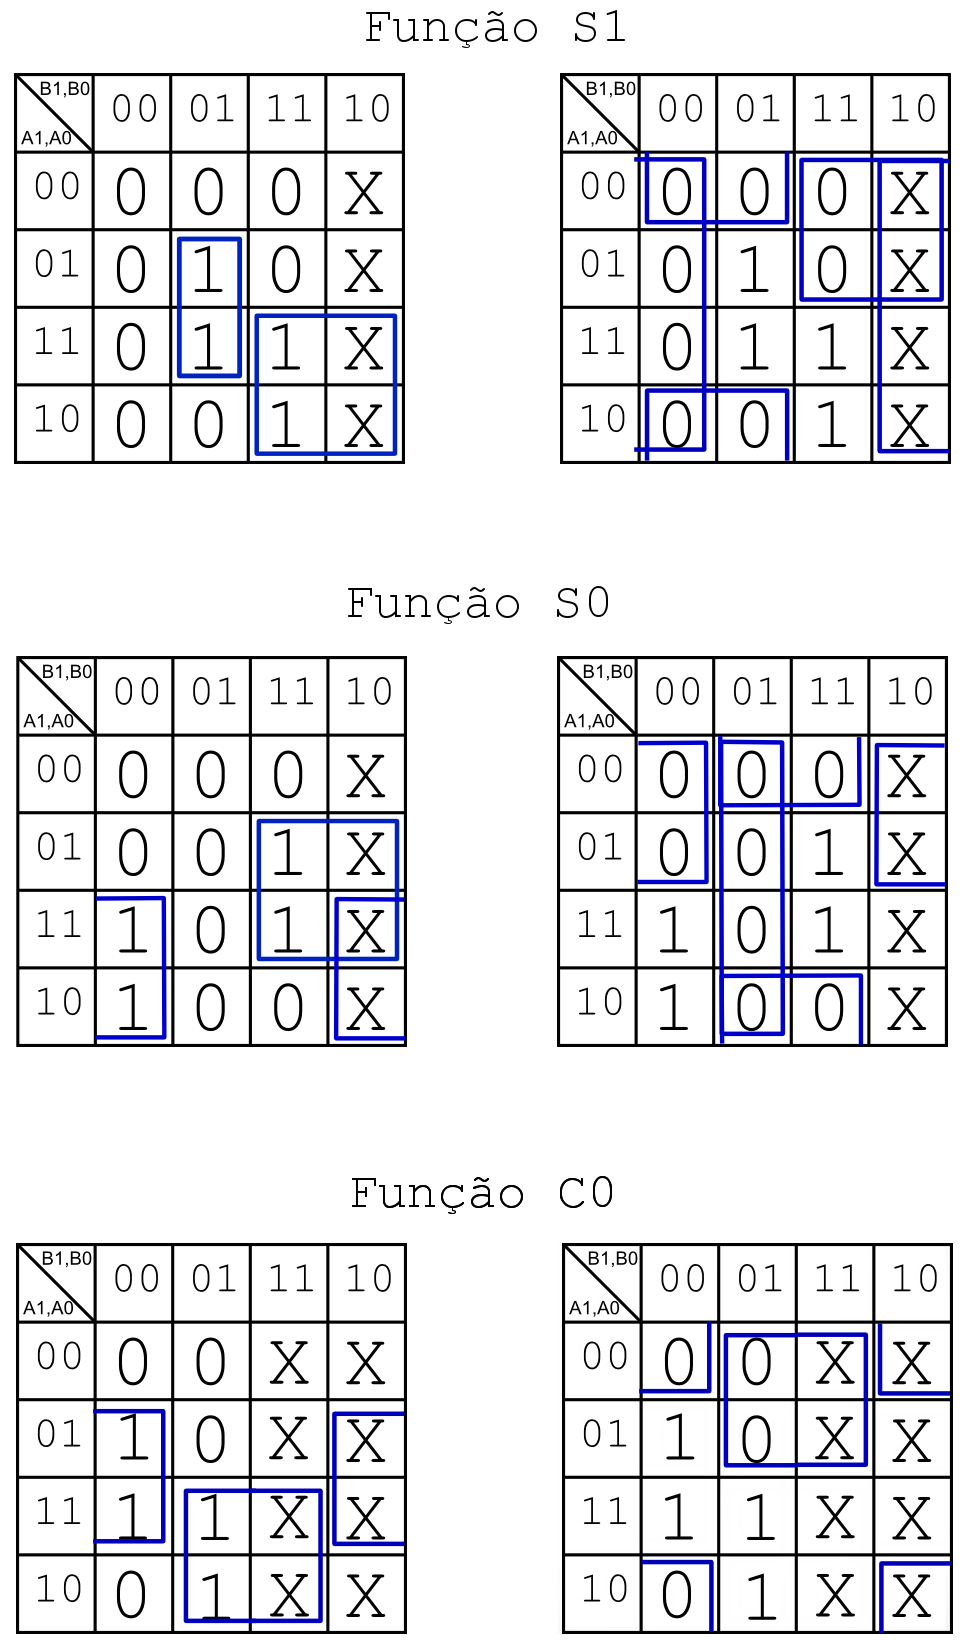
\includegraphics[scale=.27]{k3x.png}
\end{center}
\end{figure}

\begin{equation}
S_1(A_1,A_0,B_1,B_0) = A_0\overline{B_1}B_0 + A_1B_1
\end{equation}
\begin{equation}
S_0(A_1,A_0,B_1,B_0) = A_1\overline{B_0}B_1 + A_0B_1
\end{equation}
\begin{equation}
C_0(A_1,A_0,B_1,B_0) = A_0\overline{B_0} + A_1B_0
\end{equation}

Alternativamente, podemos expressá-las como produto de somas tendo em conta os quadros com implicados marcados, obtendo:


\begin{equation}
S_1(A_1,A_0,B_1,B_0) = (B_0)(A_1+\overline{B_1})(A_0+B_1)
\end{equation}
\begin{equation}
S_0(A_1,A_0,B_1,B_0) = (B_1+\overline{B_0})(A_1+\overline{B_0})(A_1+B_0)
\end{equation}
\begin{equation}
C_0(A_1,A_0,B_1,B_0) = (A_0+B_0)(A_1+\overline{B_0})
\end{equation}

\pagebreak

\subsection{Funções a construir}

Sendo os nossos números 79144 e 78811 respetivamente então:

\begin{equation}
78811 + 79144 = 157955
\end{equation}
\begin{equation}
157955/3 = 52651 + 2/3
\end{equation}

Sendo o último algarismo de um número inteiro em base três dado pelo resto
da primeira divisão desse número por três, podemos ver na operação aritmética
apresentada em (8) que o algarismo menos significativo da soma dos nossos números
é 2. Logo, apenas realizaremos a função S\textsubscript{1} e C\textsubscript{0}. 

\subsection{Transformação das expressões algébricas}

\subsubsection{De forma a serem concretizadas com portas NAND-2, NAND-3 e NOT}
\begin{enumerate}
\item A partir da forma disjuntiva
\begin{equation}
\begin{split}
S_1(A_1,A_0,B_1,B_0) & = A_0\overline{B_1}B_0 + A_1B_1 \\
                     & = \overline{\overline{((A_0\overline{B_1}B_0)}
                         ~\overline {(A_1B_1))}}  \\  
\end{split}
\end{equation}
\begin{equation}
\begin{split}
C_0(A_1,A_0,B_1,B_0) & = A_0\overline{B_0} + A_1B_0 \\
                     & = \overline{\overline{((A_0 \overline{B_0})}
                         ~\overline{(A_1 B_0))}}  \\   
\end{split}
\end{equation}
Requisitos de implementação:
\begin{enumerate}
    \item 1x NAND-3
    \item 5x NAND-2
    \item 2x NOT
  \end{enumerate}
\item A partir da forma conjutiva
\begin{equation}
\begin{split}
S_1(A_1,A_0,B_1,B_0) & = B_0~(A_0+B_1)~(\overline{B_1}+A_1) \\
                     & = \overline{\overline{B_0~\overline{\overline{(A_0}~\overline{B_1)}}
                     ~\overline{(B_1~\overline{A_1)}}}} \\
\end{split}
\end{equation}
\begin{equation}
\begin{split}
C_0(A_1,A_0,B_1,B_0) & = (A_0+B_0)~(A_1+\overline{B_0}) \\
                     & = \overline{\overline{\overline{\overline{(A_0}~\overline{B_0)}}
                     ~\overline{\overline{(A_1}~B_0)}}} \\
\end{split}
\end{equation}

\pagebreak
Requisitos de implementação:
\begin{enumerate}
    \item 1x NAND-3
    \item 5x NAND-2
    \item 6x NOT
  \end{enumerate}
\end{enumerate}
\subsubsection{De forma a serem concretizadas com portas NOR-2, NOR-3 e NOT}
\begin{enumerate}
\item A partir da forma disjuntiva
\begin{equation}
\begin{split}
S_1(A_1,A_0,B_1,B_0) & = A_0\overline{B_1}B_0 + A_1B_1 \\
                     & = \overline{\overline{\overline{\overline{(A_0} + B_1 + 
                         \overline{B_0)}}+\overline{\overline{(A_1} + \overline{B_1)}}}}  \\   
\end{split}
\end{equation}
\begin{equation}
\begin{split}
C_0(A_1,A_0,B_1,B_0) & = A_0\overline{B_0} + A_1B_0 \\
                     & = \overline{\overline{\overline{\overline{(A_0} + B_0)} 
                         + \overline{\overline{(A_1} + \overline{B_0)}}}}  \\   
\end{split}
\end{equation}
\begin{enumerate}
    \item 1x NOR-3
    \item 5x NOR-2
    \item 6x NOT
  \end{enumerate}

\par
\item A partir da forma conjutiva
\begin{equation}
\begin{split}
S_1(A_1,A_0,B_1,B_0) & = (B_0)(A_1+\overline{B_1})(A_0+B_1) \\
                     & = \overline{\overline{B_0}+\overline{(A_1+\overline{B_1)}}
                         +\overline{(A_0+B_1)}}\\
\end{split}
\end{equation}
\begin{equation}
\begin{split}
C_0(A_1,A_0,B_1,B_0) & = (A_0+B_0)(A_1+\overline{B_0}) \\
                     & = \overline{\overline{(A_0+B_0)}+\overline{(A_1+\overline{B_0)}}}\\
\end{split}
\end{equation}

Requisitos de implementação:
\begin{enumerate}
    \item 1x NOR-3
    \item 5x NOR-2
    \item 2x NOT
  \end{enumerate}
\end{enumerate}

\subsection{Diagrama Lógico}

Das várias opções analisadas em cima, optámos pela implementação com portas NAND a partir da forma disjuntiva, necessitando apenas de duas portas NOT, cinco NAND-2 e um NAND-3. Seguiremos assim o diagrama apresentado na Figura 2.
\begin{figure}[h]
\caption{Diagrama Lógico}
\begin{center}
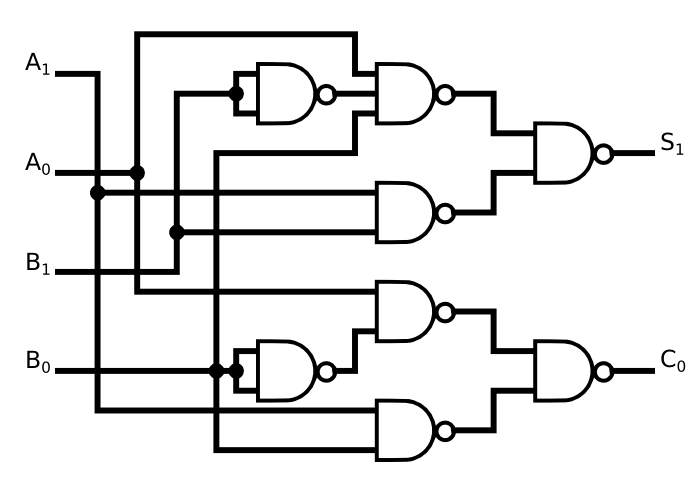
\includegraphics[scale=0.45]{SD_logi.png}
\end{center}
\end{figure}

\subsection{Valor Lógico não especificado}

Segundo as expressões optadas, na situação A=1 e B=2, de valor não determinado, terão valores lógicos:

\begin{equation}
\begin{split}
S_1(0,1,1,0) & = 1\cdot\overline{1}\cdot0 + 0\cdot1\\
                     & = 0 + 0 = 0  \\  
\end{split}
\end{equation}
\begin{equation}
\begin{split}
C_0(0,1,1,0) & = 1\cdot\overline{0} + 0\cdot0 \\
                     & = 1\cdot1 + 0 = 1  \\   
\end{split}
\end{equation}

\subsection{Esquema Eléctrico}
Para a realização deste circuito segundo o logigrama previamente apresentado, serão necessários três circuitos integrados: um SN74LS10, com portas NAND-3, e dois SN74LS00. De forma a necessitarmos apenas destes três CIs, concretizaremos cada porta NOT juntando as entradas de uma porta NAND-2. Isto é necessário pois precisamos de 5 portas NAND-2. Caso utilizássemos portas NOT, utilizaríamos 4 CIs, pois precisaríamos dois SN74LS00 de qualquer forma. A não ser que utilizássemos uma porta NAND-3 como NAND-2, porém considerámos mais simples a solução apresentada.

\begin{figure}[h]
\caption{Esquema Eléctrico}
\begin{center}
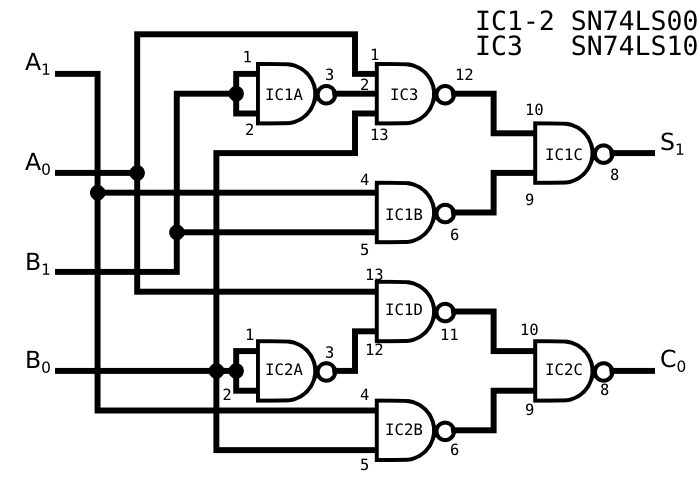
\includegraphics[scale=0.65]{SD_elect.png}
\end{center}
\end{figure}

\section{Montagem e Teste}
\subsection{Montagem}
Montou-se o circuito na {\it breadboard} utilizando os circuitos requisitados.
\subsection{Utilização da Ponta de Prova}
%\vspace*{10\baselineskip}
\pagebreak
\subsection{Teste do circuito}

\begin{table}
\centering
%\begin{tabular}{ || c  c | c c || c | c || c | c || }
\begin{tabularx}{1.1\textwidth}{|| >{\setlength\hsize{1\hsize}\centering}X >{\setlength\hsize{1\hsize}\centering}X | >{\setlength\hsize{1\hsize}\centering}X >{\setlength\hsize{1\hsize}\centering}X || >{\setlength\hsize{1\hsize}\centering}X >{\setlength\hsize{1\hsize}\centering}X || >{\setlength\hsize{1\hsize}\centering}X  | c ||}
%\begin{tabularx}{\textwidth}{||{\centering}X {\centering}X}|{\centering}X {\centering}X} ||{\centering}X {\centering}X}|| {\centering}X {\centering}X}
\hline 
\multicolumn{4}{||c||}{Valores de entrada} & \multicolumn{2}{c||}{Valores Esperados} & \multicolumn{2}{c||}{Valores de Saída} \\
  \hline
A\textsubscript{1} & A\textsubscript{0} & B\textsubscript{1} & B\textsubscript{0} & S\textsubscript{1} & C\textsubscript{0} & S\textsubscript{1} & C\textsubscript{0} \\ \hline
0   & 0  & 0  & 0  & L  & L && \\ \hline
0   & 0  & 0  & 1  & L  & L &&\\ \hline
0   & 0  & 1  & 0  & X  & X  &&\\ \hline
0   &  0  & 1   & 1   & L  & X &&\\ \hline
0   &  1  &  0  & 0   & L  & H  &&\\ \hline
0   &  1  &  0  & 1   & H  & L  &&\\ \hline
0   &  1  &  1  & 0   & X  & X  &&\\ \hline
0   &  1  &  1  & 1   & L  & X  &&\\ \hline
1   &  0  &  0  & 0   & L  & L  &&\\ \hline
1   &  0  &  0  & 1   & L  & H  &&\\ \hline
1   &  0  &  1  & 0   & X  & X  &&\\ \hline
1   &  0  &  1  & 1   & H  & X  &&\\ \hline
1   &  1  &  0  & 0   & L  & H  &&\\ \hline
1   &  1  &  0  & 1   & H  & H  &&\\ \hline
1   &  1  &  1  & 0   & X  & X  &&\\ \hline
1   &  1  &  1  & 1   & H  & X  &&\\ \hline
\end{tabularx}
%\end{tabular} 
\caption{Tabela de Teste}
\end{table}
\vspace*{7\baselineskip}
\subsubsection{Comentário dos resultados}
%\vspace*{15\baselineskip}
\pagebreak
\section{Conclusão}
\par


\end{document}

-----------> footnotes
